The algorithm presented in this work is available as an open source implementation. This implementation forms a key part in the Pithya \cite{pithya} parameter synthesis tool for ODE based biochemical models. The source code and manual are also provided as digital appendices.

In this chapter, we discuss the architecture and characteristics of this implementation.

\section{Pithya core overview}

The Pithya tool has two main components: \emph{graphical user interface} and the \emph{core engine}. Here, we are concerned only about the core engine.

The core engine is implemented in an object-oriented manner using the Kotlin programming language (compiles to standard JVM byte-code). Furthermore, the engine can use the Microsoft Z3 SMT solver \cite{z3} for decisions about the parameter formulae.

The core engine itself is also divided into several modules:

\begin{itemize}
	\item \textbf{Temporal Logic Module} This module is responsible for parsing the \ac{HUCTLp} formulae and performing necessary transformations to ensure the formulae use only the supported set of operators. The input format of the \ac{HUCTLp} formulae is specified as an ATLR4 \cite{antlr} grammar.
	\item \textbf{Parameter Synthesis Module} The main module containing the algorithm itself with abstract definitions of the necessary data structures such as solver, state map or model.
	\item \textbf{ODE Model Module} Defines a parser for the \texttt{.bio} ODE model files and a set of solvers, successor generators and state maps that work with ODE models.
	\item \textbf{CLI Front-end} Provides a command line interface, combining the functionality of all modules into one executable.
\end{itemize}

In the following sections we will discuss these modules in detail.

\section{Parameter Synthesis Module}

\subsection{States and parameter formulae representation}

Before describing the components of the parameter synthesis module, we have to define the basic requirements it poses on anyone willing to use it:

\begin{itemize}
	\item States of the \ac{PDTS} all have unique (even across fragments) integer identifiers from a continuous range. This allows easier partitioning and provides room for interesting optimisations.
	\item On the other hand, the parameter formula representation is fully generic, allowing the user to choose whatever domain specific representation suits their needs. The only requirement is that the user provides a solver capable of performing basic operations required by the algorithm (discussed later in this section).
\end{itemize}

\subsection{User-implemented interfaces}

Now that we have described how the parameter synthesis module approaches states and parameters, we can describe basic interfaces that need to be implemented by potential users. Here, we provide the list of all of these interfaces with short descriptions of their functionality. However, the implementations have to adhere to a set of required invariants and synchronization rules in order for the algorithm to be valid, therefore we refer the reader to the source code documentation for more detailed information about each interface.

\begin{itemize}
	\item \texttt{StateMap} State map is a simple map interface which provides a way to represent the state—parameter mapping used when computing the assumption function. However, as opposed to the assumption function, \texttt{StateMap} is a general purpose interface used throughout the code whenever a state—parameter collection is needed (successor/predecessor representation, communication, etc.). It is immutable by default, however there is a mutable variant which is used to represent incomplete results. For the list of available implementations, see code documentation.
	
	\item \texttt{Solver} The solver should be capable of providing basic constants ($\ttrue, \ffalse$) and performing standard operations such as: Conjunction, disjunction, complement (negation), test for emptiness (satisfiability) and formula simplification. These operations are then used to implement more complex, algorithm specific operations. User is also free to override these default implementations assuming a more efficient alternative is available. Finally, each solver should be able to serialize a parameter constraint into a byte buffer so that it can be safely transferred between fragments. Additionally, the module provides sample explicit solvers based on standard collections. These usually don't scale very well with increasing number of parameter valuations, but provide a good starting point for implementing and debugging more complex solvers (for full list, see code documentation).
	
	\item \texttt{Partition} Combining the \ac{PDTS} fragment with its partition function, the \texttt{Partition} interface provides the total amount of fragments, current fragment identifier, methods for obtaining predecessors and successors of a specific state plus the ability to evaluate atomic propositions.
	
	Assuming the user does not want to provide his own partition function, they can implement a \texttt{Model} interface, which is a simplified version of the \texttt{Partition} which provides only the successor/predecessor generator and proposition evaluation. The \texttt{Model} can then be wrapped into one of the predefined partition functions:
	
	\begin{itemize}
		\item \texttt{SingletonPartition} Partition function maps all states to a single fragment. Useful for debugging or working in single threaded environment.
		\item \texttt{HashPartition} Partition which assigns states to a predefined number of fragments using an integer modulus as a hash function. It provides good levels of uniformity and concurrency, however, usually also requires a lot of communication.
		\item \texttt{UniformPartition} A uniform partition divides the states into equally sized intervals and assigns each fragment one interval. It provides good uniformity and assuming the identifiers of state neighbours are also numerically close to the identifier of the original state, it should provide low communication overhead. However, in cases when the communication cost is low, the better concurrency of the \texttt{HashPartition} can result in faster computation.
		\item \texttt{BlockPartition} A block partition is a hybrid between the \texttt{UniformPartition} and the \texttt{HashPartition}. The partition function will divide the state space into equally sized intervals, while each fragment is assigned a predefined number of intervals.
	\end{itemize}

	Apart from the predefined partitions, the parameter synthesis module also provides a very basic explicit model implementation, which can be useful for debugging, testing and creating toy examples (it is used as a model implementation for the validity testing).

	\item \texttt{Channel} Responsible for communication between fragments, functionality of \texttt{Channel} maps almost directly to the \textsc{Communicate} procedure in the algorithm pseudocode. The communication relies on serialization into byte buffers.
	
	The module provides two basic implementations:
	
	\begin{itemize}
		\item \texttt{SingletonChannel} Channel used for single threaded workloads with no ability to communicate.
		\item \texttt{SharedMemChannel} Channel which directly passes the byte buffers between fragments managed by the same virtual machine.
	\end{itemize}

	As you can see, no truly distributed channel is provided directly by the module. Users should provide their own channel based on the distributed environment where the algorithm is running.

\end{itemize}

\subsection{Module work flow}

\begin{figure}[]
	\centering
	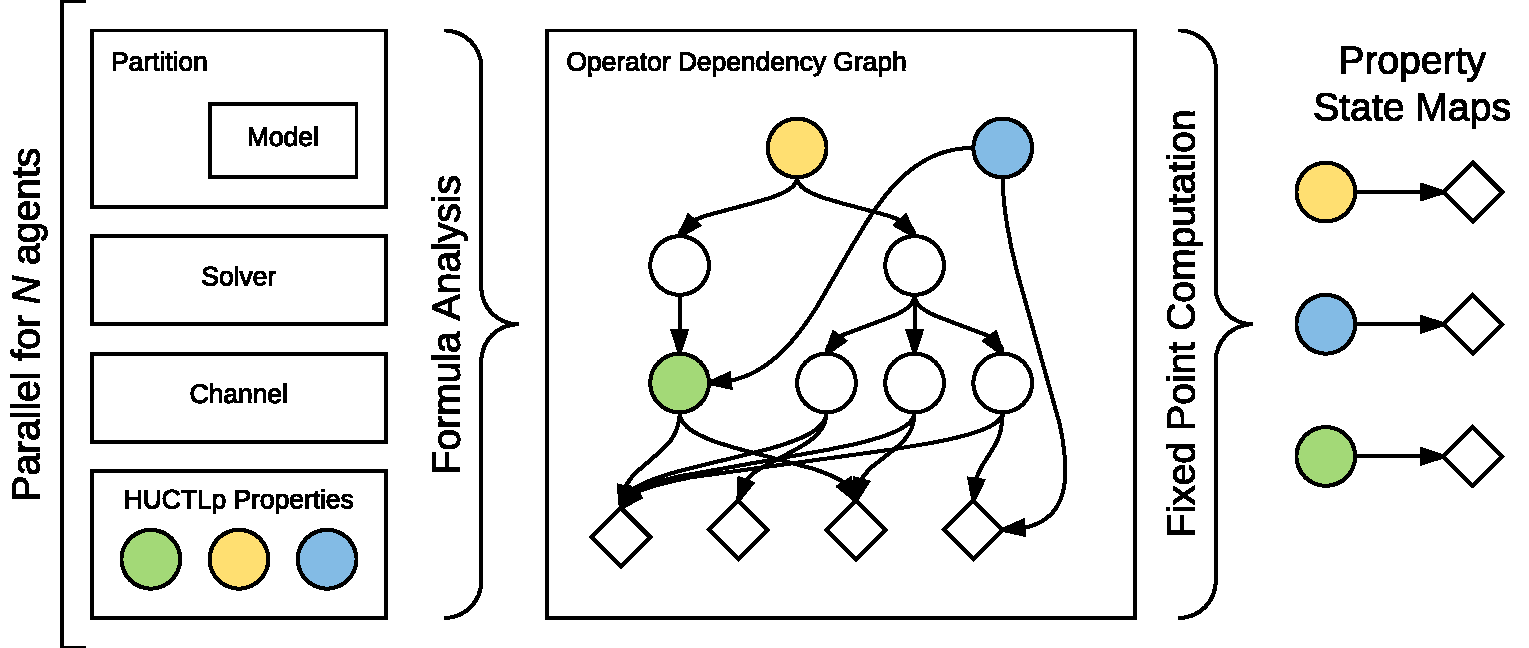
\includegraphics[scale=0.45]{media/core_workflow.pdf}
	\caption{Work flow of the main parameter synthesis module. Circles represent \ac{HUCTLp} operator objects, diamonds \texttt{StateMap}s. }
	\label{fig:core_workflow}
\end{figure}

With all necessary data structures in place, the parameter synthesis engine accepts a set of investigated \ac{HUCTLp} properties and is ready to perform the main procedure. The work flow is depicted in figure \ref{fig:core_workflow}.

The implementation starts by constructing a dependency graph based on the provided \ac{HUCTLp} properties. Each node in the graph is represented by a special operator object which implements the logic of the semantic function $\mathcal{C}$ for one specific \ac{HUCTLp} operator. 

This construction ensures that whenever two properties share a common sub-formula, it is only computed once. Furthermore, this construction also unrolls the state variable valuation, so that for example a property $\hctlAt{x} \varphi$ is represented as $|\dtsS|$ distinct operators, depending on the value of $x$. 


This allows us to ensure that unused valuations don't create unnecessary operators. A good example of such case is a formula $\hctlBind{x} \ctlA\ctlF (\neg x \land \ctlE\ctlF p)$ where $p$ is some atomic proposition. In this case, $\ctlE\ctlF$ is independent on the valuation of $x$, and therefore can be represented by a single operator node in the dependency graph, while the $\ctlA\ctlF$ is unrolled into multiple operators depending on the value of $x$.

Another important optimisation this construction allows is canonisation of the state variable names. This means that if you consider a formula such as $[\hctlBind{x} \ctlA\ctlF x] \lor [\hctlExists{y} (\ctlA \ctlF y \land \neg y)]$, both $\ctlA\ctlF x$ and $\ctlA\ctlF y$ are resolved as the same operator object and are computed only once. 

After the operator dependency graph is constructed, the fixed point algorithm iteratively processes operators in the graph, starting from the smallest (propositions). Multiple operators can be even processed concurrently, assuming their dependencies are already computed.  

As a result of this operation, user obtains a set of \texttt{StateMap}s which represent the parameter synthesis result for the local states of the fragment for each requested property, as depicted in the third part of the work flow figure.

\section{ODE Model Module}


\begin{figure}[]
	\centering
	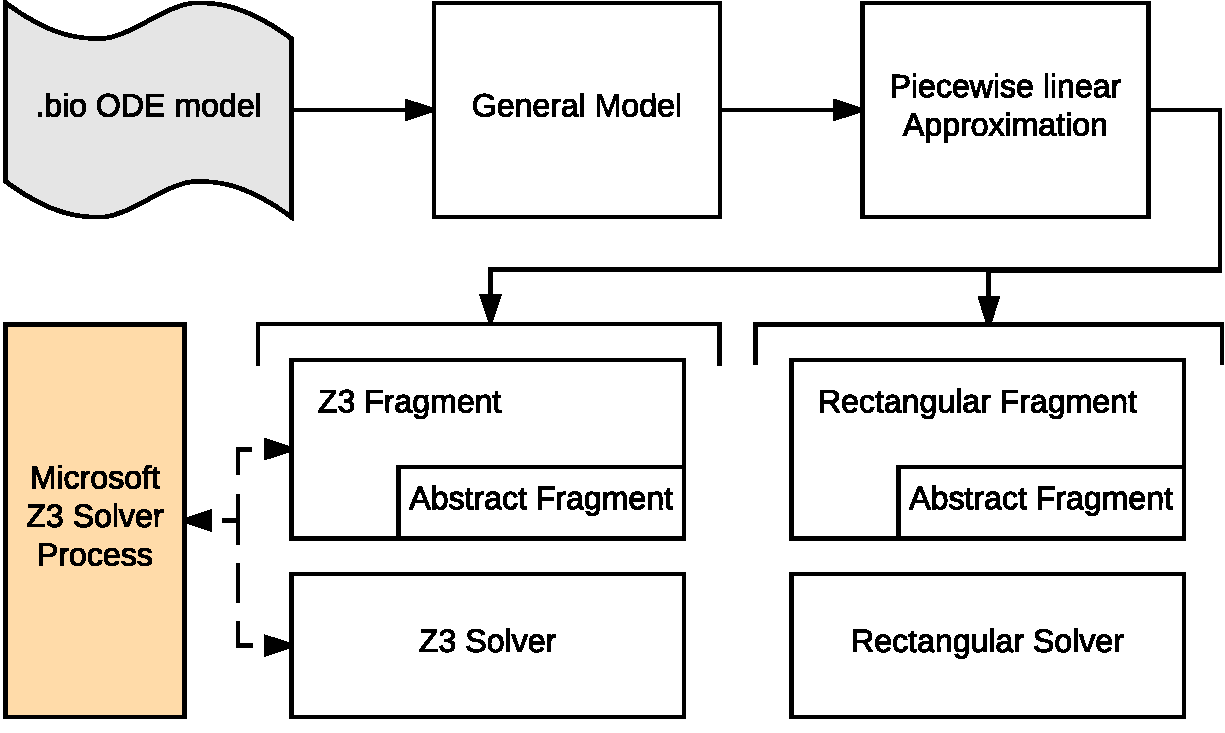
\includegraphics[scale=0.45]{media/ode_workflow.pdf}
	\caption{Work flow of the ode module module. The usage of a specific fragment implementation depends on the properties of the model. }
	\label{fig:ode_workflow}
\end{figure}

The ODE model module provides implementations for working with various types of models based on ordinary differential equations. It relies on the abstraction procedure described in \cite{abs, absOverview} when transforming the continuous equations into a discrete state space. The models are originally represented using a .bio model format (grammar provided in ANTLR4 syntax in the digital appendix) and this module is responsible for parsing the model file, computing the piecewise linear approximation and transforming the model into \ac{PDTS} fragments that can be then used by the main parameter synthesis module. The module also provides appropriate solvers for the supported model types.	

The work flow of this process, with all of it's main components is depicted in figure \ref{fig:ode_workflow}. After the piecewise linear approximation is constructed, the model is analysed for relationships between parameters and an appropriate parameter representation is chosen.

\texttt{Rectangular Model} and the corresponding \texttt{Rectangular Solver} are chosen when the parameters are fully independent (at most one parameter per equation). This type of parameter representation uses a set of hyper-rectangles to encode the parameter constrain and is fairly straightforward and efficient.

\texttt{Z3 Model} and \texttt{Z3 Solver} are then used for more complex models. In this case, the parameter constrains are represented directly as Microsoft Z3 compatible formulae and the SMT solver is directly responsible for deciding satisfiability and formula simplification. This is facilitated by directly interfacing with a Z3 process running in interactive mode. Z3 also provides a direct API for common programming languages. However, we choose not to use this, because it causes problems with parallelism on multi-core machines. 

At the time of writing, Z3 was designed in a way that even for formulae which belong to completely separate contexts, some non-trivial synchronisation is performed. This synchronisation then significantly cripples the parallel execution to a point where adding more concurrent workers actually slows down the execution significantly. Having a set of independent (at the system level) solver processes then enables us to scale the execution on multi-core machines, even though it introduces more overhead and complexity to the whole program.

Finally, this module also provides an \texttt{Abstract Model} class which implements general logic for generating transitions in ODE based models. One can use this class to quickly implement new model variants. All that needs to be provided is a method producing a parameter constrain under which is a given equation at a given vertex positive or negative (corresponding to a positive or negative derivation). Other logic and optimisations (caching, etc.) is then handled solely by the abstract implementation. Naturally, an appropriate solver also has to be provided.

\section{Command line frontend}

\begin{figure}[]
	\centering
	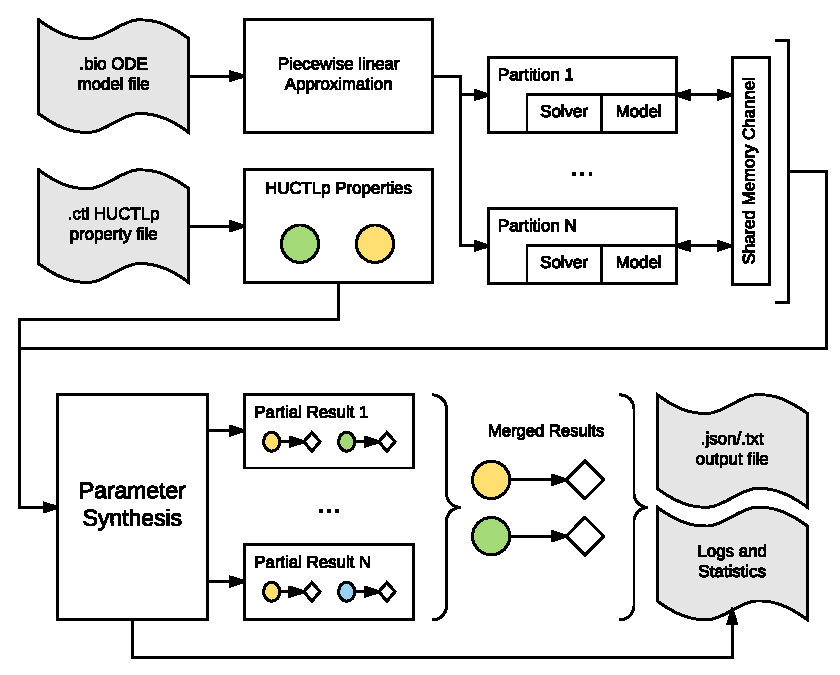
\includegraphics[scale=0.9]{media/cli_workflow.pdf}
	\caption{Work flow of the command line front-end. }
	\label{fig:cli_workflow}
\end{figure}

The command line front-end connects all these modules into one package with a well defined input and output. Schematic description of this module is given in Figure \ref{fig:cli_workflow}.

The process starts by parsing given input files and creating $N$ independent partitions connected using a shared memory communication channel. These data structures are then passed into the parameter synthesis engine.

As soon as the parameter synthesis is finished, the front-end module obtains $N$ partial results from the synthesis engine. These partial results are then merged into one general result set. Finally, the result set can be exported using two supported output formats. First format provides export into a machine readable .json file, suitable for further post-processing or visualisations. Second format provides a more human readable text format, which can be useful when debugging or working with simple models.

The actual content of both formats depends on the type of parameter representation used by the model. When working with hyper-rectangular parameter representation, a parameter constrain is represented using a suitable multi dimensional array interpreted directly as a set of hyper-rectangles. On the other hand, when working with the pure SMT approach, a parameter constrain is represented as a SMT-LIB 2 formula \cite{smtlib}.

Finally, a set of diagnostic and benchmarking data is collected during the computation. These include the amount and frequency of data transfers between partitions (to monitor possible communication bottlenecks) and the average solver throughput (corresponds to the complexity of parameter constrains which were encountered during the computation). These data are generally printed directly to the standard output or can be easily redirected into a separate file.

For a detailed description of the command line arguments accepted by the front-end module, see the tool manual provided as a digital appendix.

